%%%% acra.tex

\typeout{Informative Path Planning with Gaussian Process Classifiers for Seafloor Exploration}

% This is the instructions for authors for ACRA.
\documentclass{article}
\usepackage{acra}
% The file acra.sty is the style file for ACRA. 
% The file named.sty contains macros for named citations as produced 
% by named.bst.

% The preparation of these files was supported by Schlumberger Palo Alto
% Research, AT\&T Bell Laboratories, and Morgan Kaufmann Publishers.
% Shirley Jowell, of Morgan Kaufmann Publishers, and Peter F.
% Patel-Schneider, of AT\&T Bell Laboratories collaborated on their
% preparation. 

% These instructions can be modified and used in other conferences as long
% as credit to the authors and supporting agencies is retained, this notice
% is not changed, and further modification or reuse is not restricted.
% Neither Shirley Jowell nor Peter F. Patel-Schneider can be listed as
% contacts for providing assistance without their prior permission.

% To use for other conferences, change references to files and the
% conference appropriate and use other authors, contacts, publishers, and
% organizations.
% Also change the deadline and address for returning papers and the length and
% page charge instructions.
% Put where the files are available in the appropriate places.


%%%%%% Start: Kelvin's Packages %%%%%% 
\usepackage{vector}  % Allows "\bvec{}" and "\buvec{}" for "blackboard" style bold vectors in maths
\usepackage{bm}
\usepackage{amsmath}
\usepackage{amssymb}
\usepackage{graphicx}
\usepackage[usenames, dvipsnames]{color} % pdfLaTeX
\renewcommand{\vec}[1]{\boldsymbol{#1}}
\newcommand\numberthis{\addtocounter{equation}{1}\tag{\theequation}}

\title{Receding Horizon Approach to Informative Seafloor Exploration using Linearised Entropy of Gaussian Process Classifiers}
% Informative Path Planning with Gaussian Process Classifiers for Seafloor Exploration
% Receding Horizon Approach to Informative Seafloor Exploration with Gaussian Process Classifiers
% Receding Horizon Approach to Informative Seafloor Exploration with Linearised Entropy of Gaussian Process Classifiers

\author{Kelvin Hsu \\ University of Sydney, Australia \\ 
Kelvin.Hsu@nicta.com.au}



\begin{document}

\maketitle

\begin{abstract}
	While seafloor bathymetry have been mapped extensively over the last century, geological and ecological observations of seafloor benthic zones only began recently. Unlike bathymetric mapping, data collection of benthic imagery requires \textit{in situ} exploration - a significantly slower and costly endeavour. An efficient exploration policy would therefore require solving the informative path planning problem. This paper investigates a receding horizon approach to the informative path planning problem using linearised entropy as the proposed acquisition function. We model the benthic environment upon five bathymetric features through Gaussian process classifiers, whose linearised entropy would be defined and derived. We compare our method to a monte carlo approach for estimating joint entropy under a prediction accuracy criterion, demonstrating advantages of the linearised entropy approach. Under the same acquisition criterion, we also show the benefits of a receding horizon approach over simpler approaches such as greedy and open loop methods. Finally, we test our method on collected benthic datasets from past AUV missions to Scott Reef, Western Australia. 
\end{abstract}

\section{Introduction}
\label{Section:Introduction}
	
	Introduce GPs \cite{GaussianProcessForMachineLearning}
%	
\section{Mapping Benthic Habitats with Gaussian Process Classifiers}
\label{Section:BenthicMapping}

		\begin{figure}[!htbp]
			\centering
				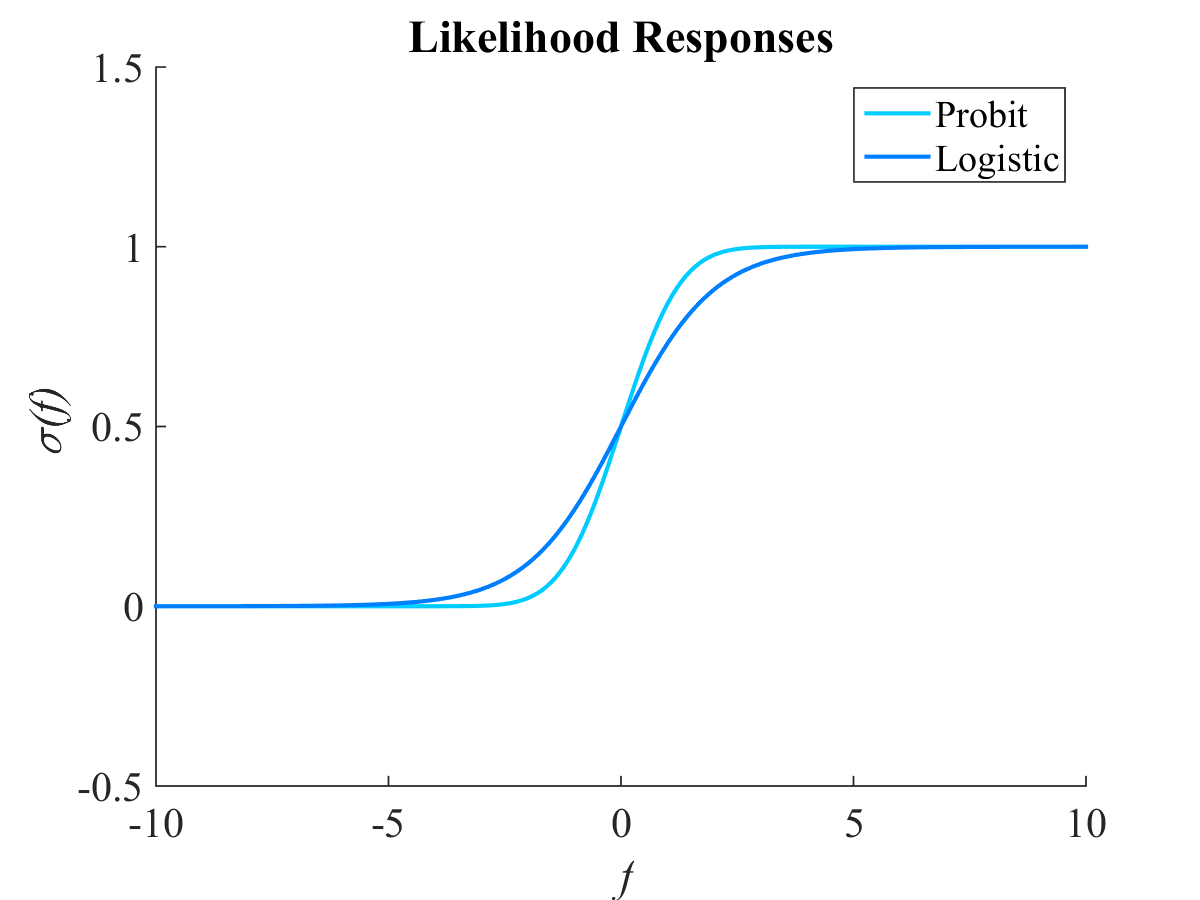
\includegraphics[width = \linewidth]{Figures/responses.png}
			\caption{Likelihood Responses}
			\label{Figure:LikelihoodResponses}
		\end{figure}
	
\section{Linearised Entropy of Gaussian Process Classifiers}
\label{Section:LinearisedEntropy}

	\subsection{Binary Classification}
	
		For binary classification, linearisation is performed on the likelihood response function.
	
		Suppose we have trained our Gaussian process classifier using Laplace approximation with respect to a training set $\mathcal{D} = \{X, \vec{y}\} = \{[ \vec{x}_{1}, \vec{x}_{2}, \dots, \vec{x}_{n}]^{T}, [y_{1}, y_{2}, \dots, y_{n}]\}$ with $n$ training points. We know that the latent function $f(\vec{x})$ is distributed as a GP with a particular predictive mean $m(\vec{x})$ and covariance $k(\vec{x}, \vec{x}')$ once conditioned on the training data \eqref{Section:LinearisedEntropy:Equation:PredictiveGP}. From here on we omit explicitly notating the training set that was conditioned upon.
		
		\begin{equation}
			f(\vec{x}) \sim \mathcal{GP}(m(\vec{x}), k(\vec{x}, \vec{x}'))
		\label{Section:LinearisedEntropy:Equation:PredictiveGP}
		\end{equation}
		
		Let $X^{\star} = [ \vec{x}^{\star}_{1}, \vec{x}^{\star}_{2}, \dots, \vec{x}^{\star}_{n^{\star}}]^{T}$ denote the collection of $n^{\star}$ query points for which inference is to be performed. Denote $\vec{f}^{\star}$ the vector of latent function values $f^{\star}_{i} = f(\vec{x}^{\star}_{i})$ at each query point. We have by definition of a GP that $\vec{f}^{\star}$ is multivariate Gaussian distributed with a corresponding means $\mu^{\star}_{i} = m(\vec{x}^{\star}_{i})$ and covariances $\Sigma^{\star}_{ij} = k(\vec{x}^{\star}_{i}, \vec{x}^{\star}_{j})$ \eqref{Section:LinearisedEntropy:Equation:PredictiveGaussianDistribution}.
		
		\begin{equation}
			\vec{f}^{\star} = [f^{\star}_{1}, f^{\star}_{2}, \dots, f^{\star}_{n^{\star}}]^{T} \sim \mathcal{N}(\vec{\mu}^{\star}, \Sigma^{\star})
		\label{Section:LinearisedEntropy:Equation:PredictiveGaussianDistribution}
		\end{equation}
			
		The binary prediction probability $\vec{\pi^{\star}}$ at the query points is obtained through passing the queried latent function random vector $\vec{f}^{\star}$ through a response function in a component wise fashion \eqref{Section:LinearisedEntropy:Equation:Response}.
		
		\begin{equation}
			\pi^{\star}_{i} = \sigma(f^{\star}_{i}) \qquad \forall i \in \{1, 2, \dots, n^{\star}\}
		\label{Section:LinearisedEntropy:Equation:Response}
		\end{equation}
		
		As a straightforward transformation of the latent vector, the predictive probability vector $\vec{\pi^{\star}}$ is thus a random vector itself. The usual procedure is then to treat the expected predition probabilities $\mathbb{E}(\vec{\pi^{\star}})$ as the posterior class probabilities for further inference. However, this discards any information regarding the joint behaviour at the query points. As a result, a measure of mutual information shared amongst the query points cannot be obtained.
		
		One straightforward approach to address this problem is to perform Monte Carlo estimation of the posterior joint distribution for class predictions via jointly sampling latent vectors from the GP, assigning class label 1 for positive latent values and -1 otherwise, and compute the Shannon entropy \cite{ShannonEntropy} from the estimated joint distribution. Aside from the relatively long computational time required for sampling enough draws for accurate joint distribution estimation, the Monte Carlo approach also has the tendency to overestimate variances at locations with low densities of training observations.
				
		Instead, we propose using the joint distribution of the predictive probabilities $\vec{\pi^{\star}}$ itself as a basis of constructing a measure of mutual information. Unlike traditional approaches where inference depends only on the expectance $\mathbb{E}(\vec{\pi^{\star}})$ such that structural information from the latent GP is compromised, we utilise also the covariance $\mathbb{V}(\vec{\pi^{\star}})$, which withholds information regarding both the latent GP and the response likelihood.
	
		\begin{figure}[!htbp]
			\centering
				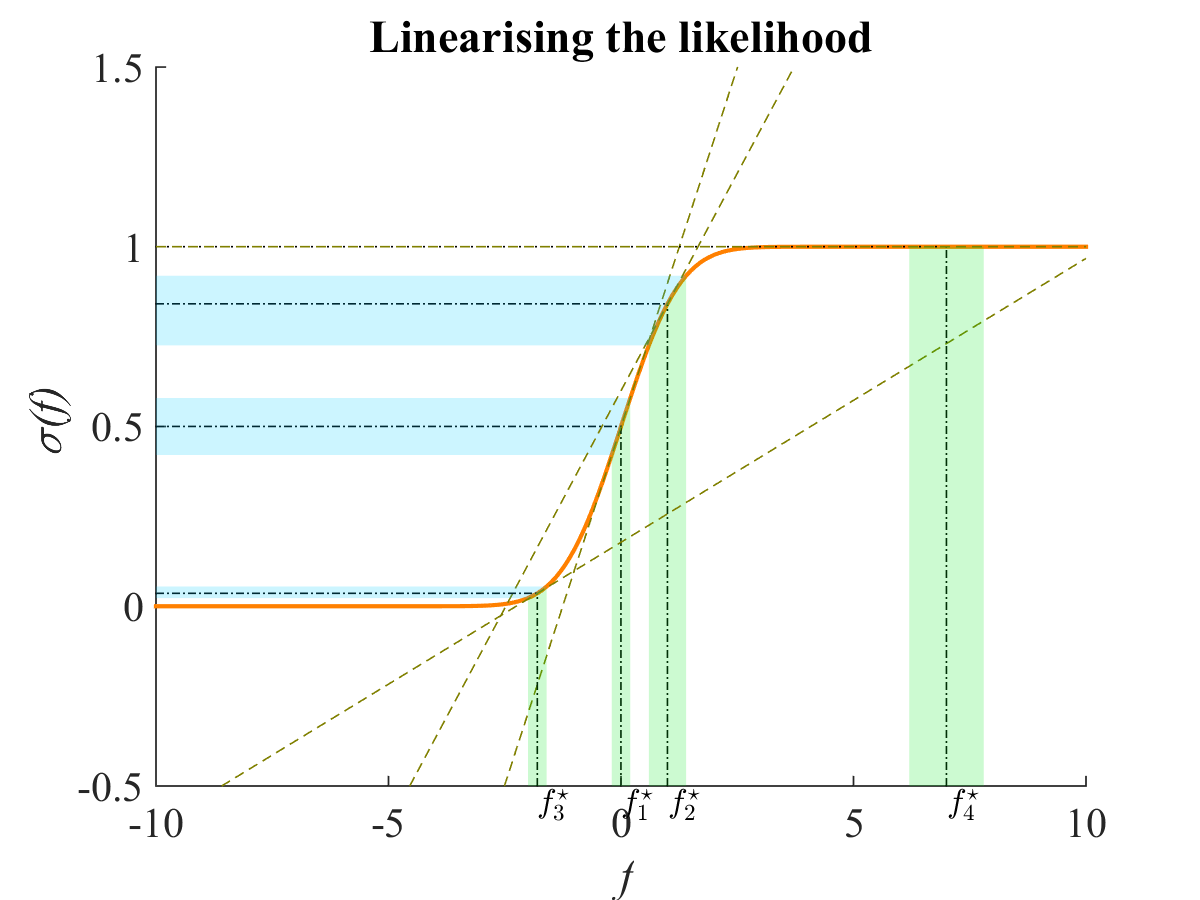
\includegraphics[width = \linewidth]{Figures/linearisation.png}
			\caption{Linearisation accuracy for a probit response: Green shade represents the latent variance while blue shade represents the predictive variance. Gold lines show local linearisation about latent expectance.}
			\label{Figure:Linearisation}
		\end{figure}
			
		As the predictive probabilities are nonlinear transformations (Figure \ref{Figure:LikelihoodResponses}) of the Gaussian distributed latent vector, they are no longer Gaussian distributed. Hence, we propose linearising the response function about the latent expectance $\bar{f}^{\star}_{i} := \mathbb{E}(f^{\star}_{i})$. Figure \ref{Figure:Linearisation} illustrates the linearisation accuracy for a probit response. Observe that points with latent expectance far away from zero translate to near zero predictive variance even under high latent variance. Linearisation is thus very accurate for those points. For points with latent expectances near zero, we require the latent variances to be sufficiently bounded for linearisation to be accurate.

		\subsubsection{Derivation}
		
			We proceed to derive the linearisation which also serves to construct the definition of linearised entropy. With first order Taylor expansion, we linearise the response about the chosen linearisation point $\bar{f}^{\star}_{i} = \mathbb{E}(f^{\star}_{i})$.
			
			\begin{equation}
				\sigma(f^{\star}_{i}) \approx \sigma_{L}(f^{\star}_{i}) := \sigma(\bar{f}^{\star}_{i}) + \sigma'(\bar{f}^{\star}_{i}) (f^{\star}_{i} - \bar{f}^{\star}_{i})
			\label{Section:LinearisedEntropy:Equation:LinearisingSigmoid}
			\end{equation}
			
			The prediction probabilities are now approximated as a linear transformation $\sigma_{L}(f)$ of the latent vector, so that it is also multivariate Gaussian distributed with expectance and covariance available in analytical form \eqref{Section:LinearisedEntropy:Equation:MomentsLinearisedSigmoid}.
			
			\begin{align*}
			\numberthis \label{Section:LinearisedEntropy:Equation:MomentsLinearisedSigmoid}
					\sigma_{L}(\vec{f}^{\star}) & \sim \mathcal{N}(\vec{\mu}^{\star}_{L}, \Sigma^{\star}_{L}) \\
					\mathbb{E}(\sigma_{L}(f^{\star}_{i})) & = \mathbb{E}(\sigma(f^{\star}_{i})) = ({\mu^{\star}_{L}})_{i} \\
					\mathbb{C}\mathrm{ov}(\sigma_{L}(f^{\star}_{i}), \sigma_{L}(f^{\star}_{j})) & =  \mathbb{C}\mathrm{ov}(\sigma(\bar{f}^{\star}_{i}) + \sigma'(\bar{f}^{\star}_{i}) (f^{\star}_{i} - \bar{f}^{\star}_{i}),\\ 
					& \qquad \;\;\;\;\; \sigma(\bar{f}^{\star}_{j}) + \sigma'(\bar{f}^{\star}_{j}) (f^{\star}_{j} - \bar{f}^{\star}_{j})) \\
					& = \sigma'(\bar{f}^{\star}_{i}) \sigma'(\bar{f}^{\star}_{j}) \mathbb{C}\mathrm{ov}(f^{\star}_{i}, f^{\star}_{j}) = ({\Sigma^{\star}_{L}})_{ij}			
			\end{align*}
			
			We then define the linearised entropy $H^{\star}_{L}$ at the query points $X^{\star}$ to be the differential entropy for which the random vector $\sigma_{L}(\vec{f}^{\star})$ holds. Since $\sigma_{L}(\vec{f}^{\star})$ is multivariate Gaussian distributed, $H_{L}$ exhibits a closed form \eqref{Section:LinearisedEntropy:Equation:LinearisedEntropy}.
			
			\begin{equation}
				H^{\star}_{L} := \frac{1}{2} \log\Big((2 \pi e)^{n^{\star}} |\Sigma_{L}|\Big)
			\label{Section:LinearisedEntropy:Equation:LinearisedEntropy}
			\end{equation}			
				
		\subsubsection{Results}
		
			\begin{figure*}[tb]
			\centering
				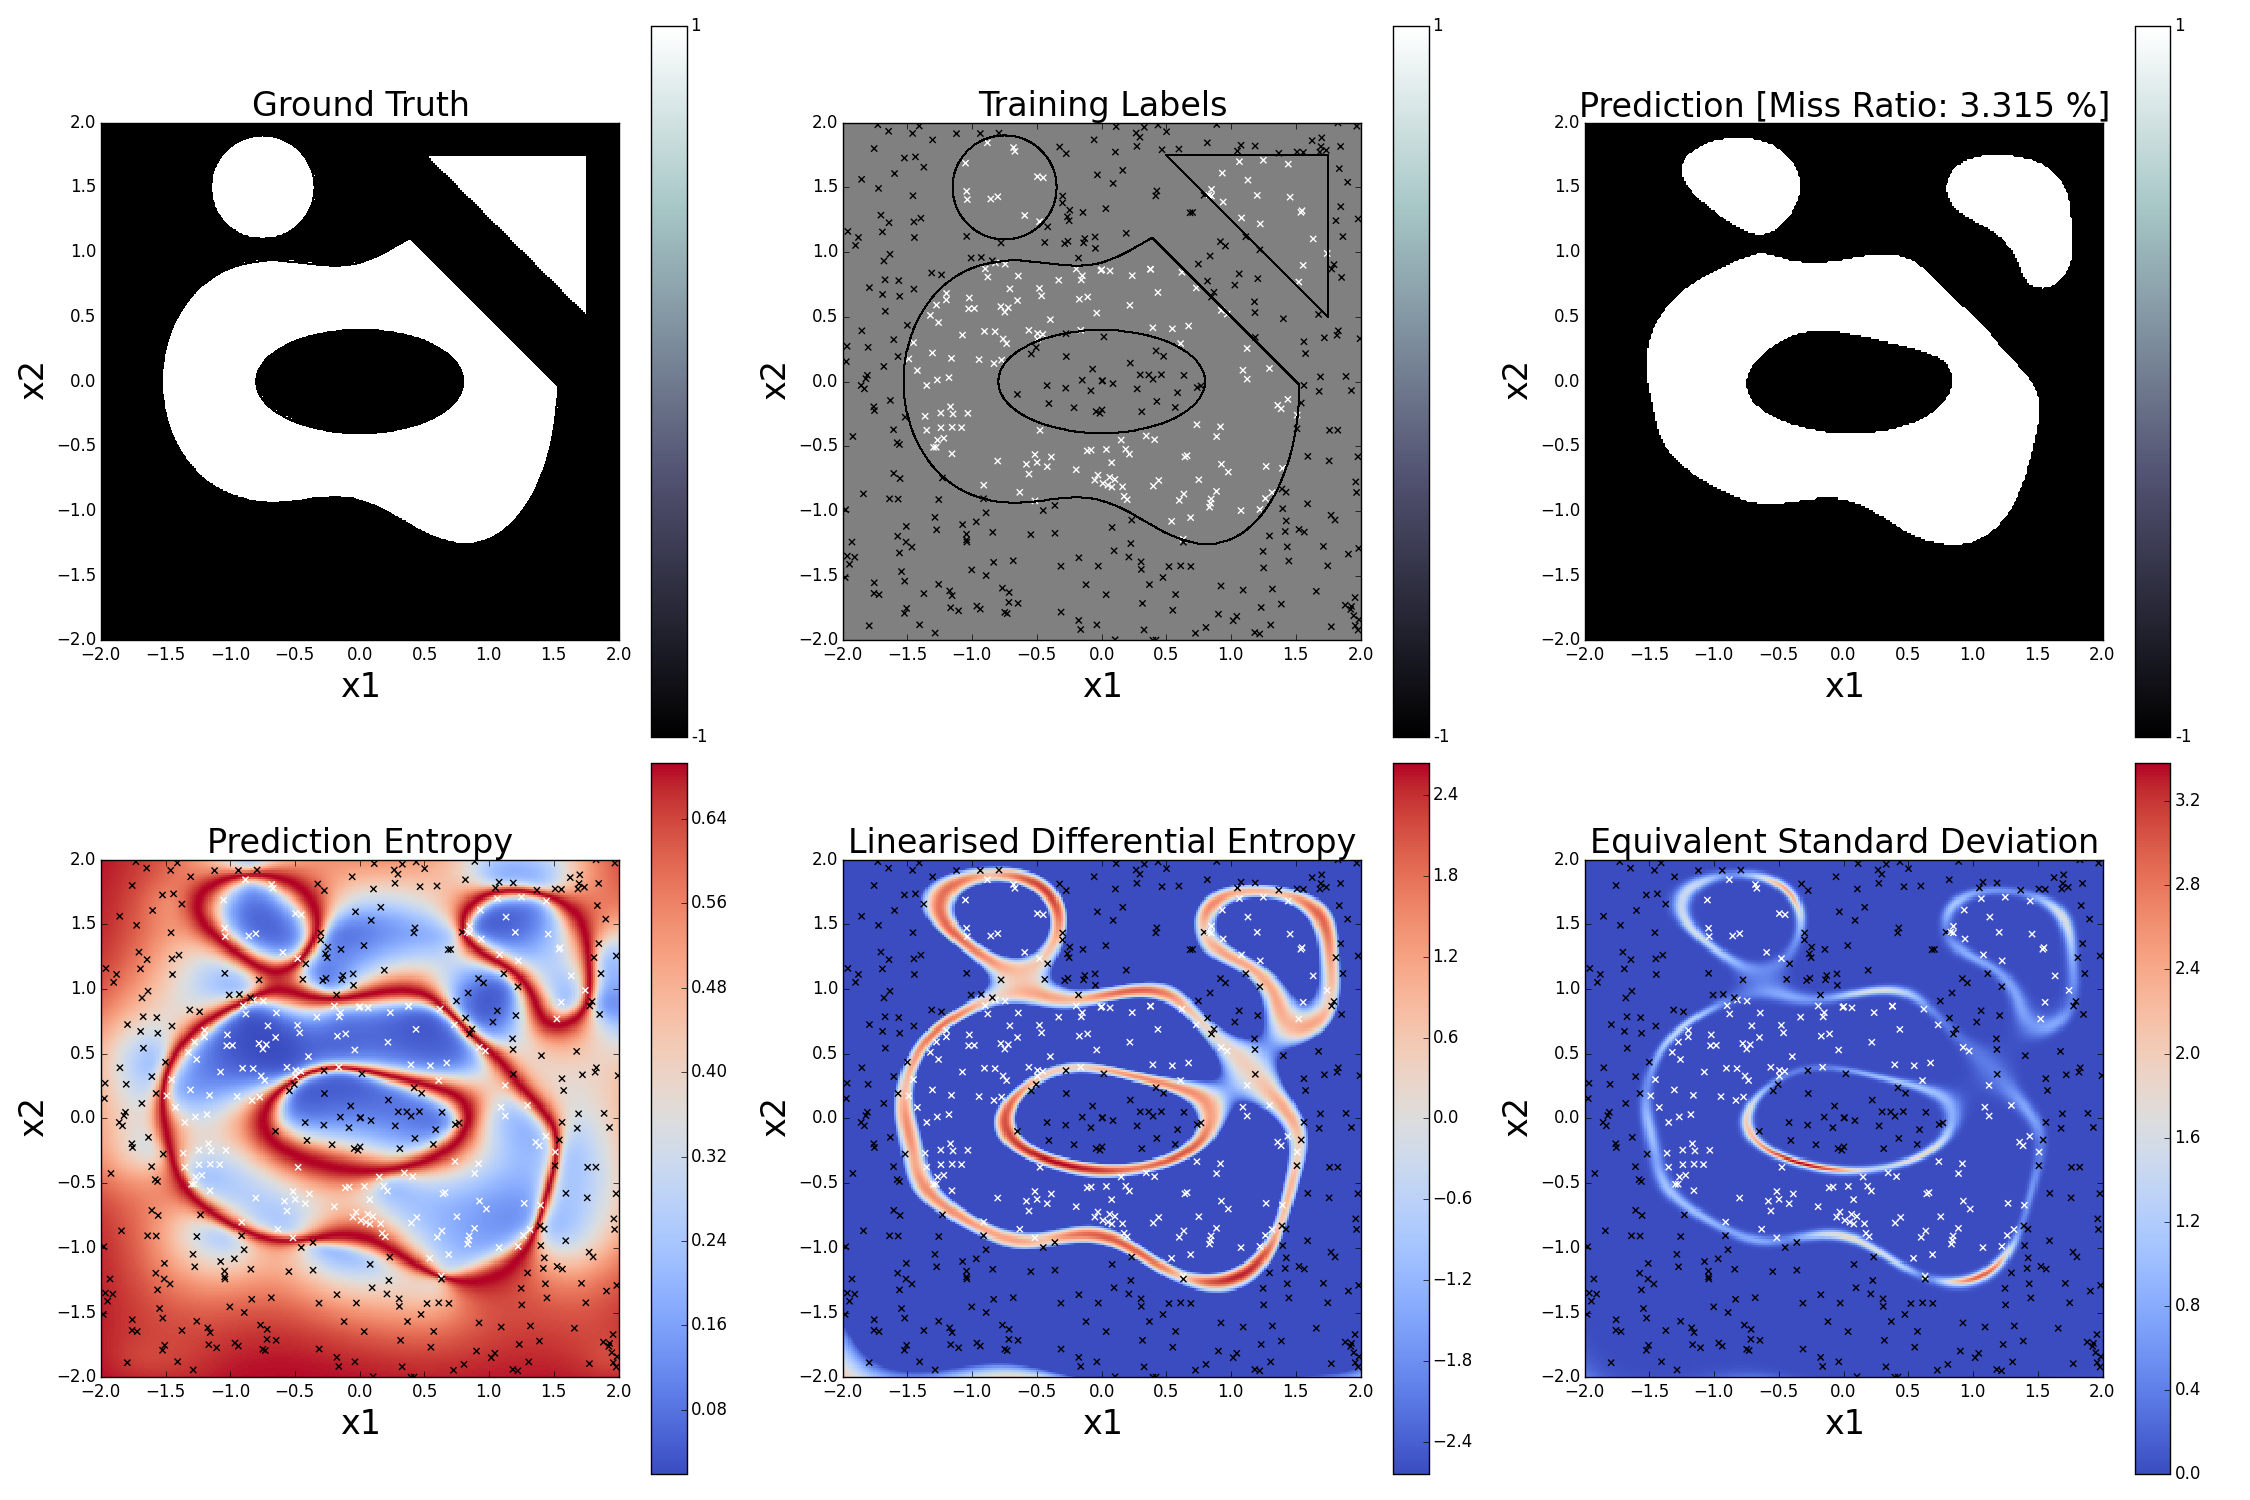
\includegraphics[width = \linewidth]{Figures/binary_linearised_entropy/Figure1.png}
			\caption{Example: Linearised Entropy for a Binary Classifier}
			\label{Figure:Results:BinaryLinearisedEntropy}
			\end{figure*}

			\begin{figure*}[tb]
			\centering
				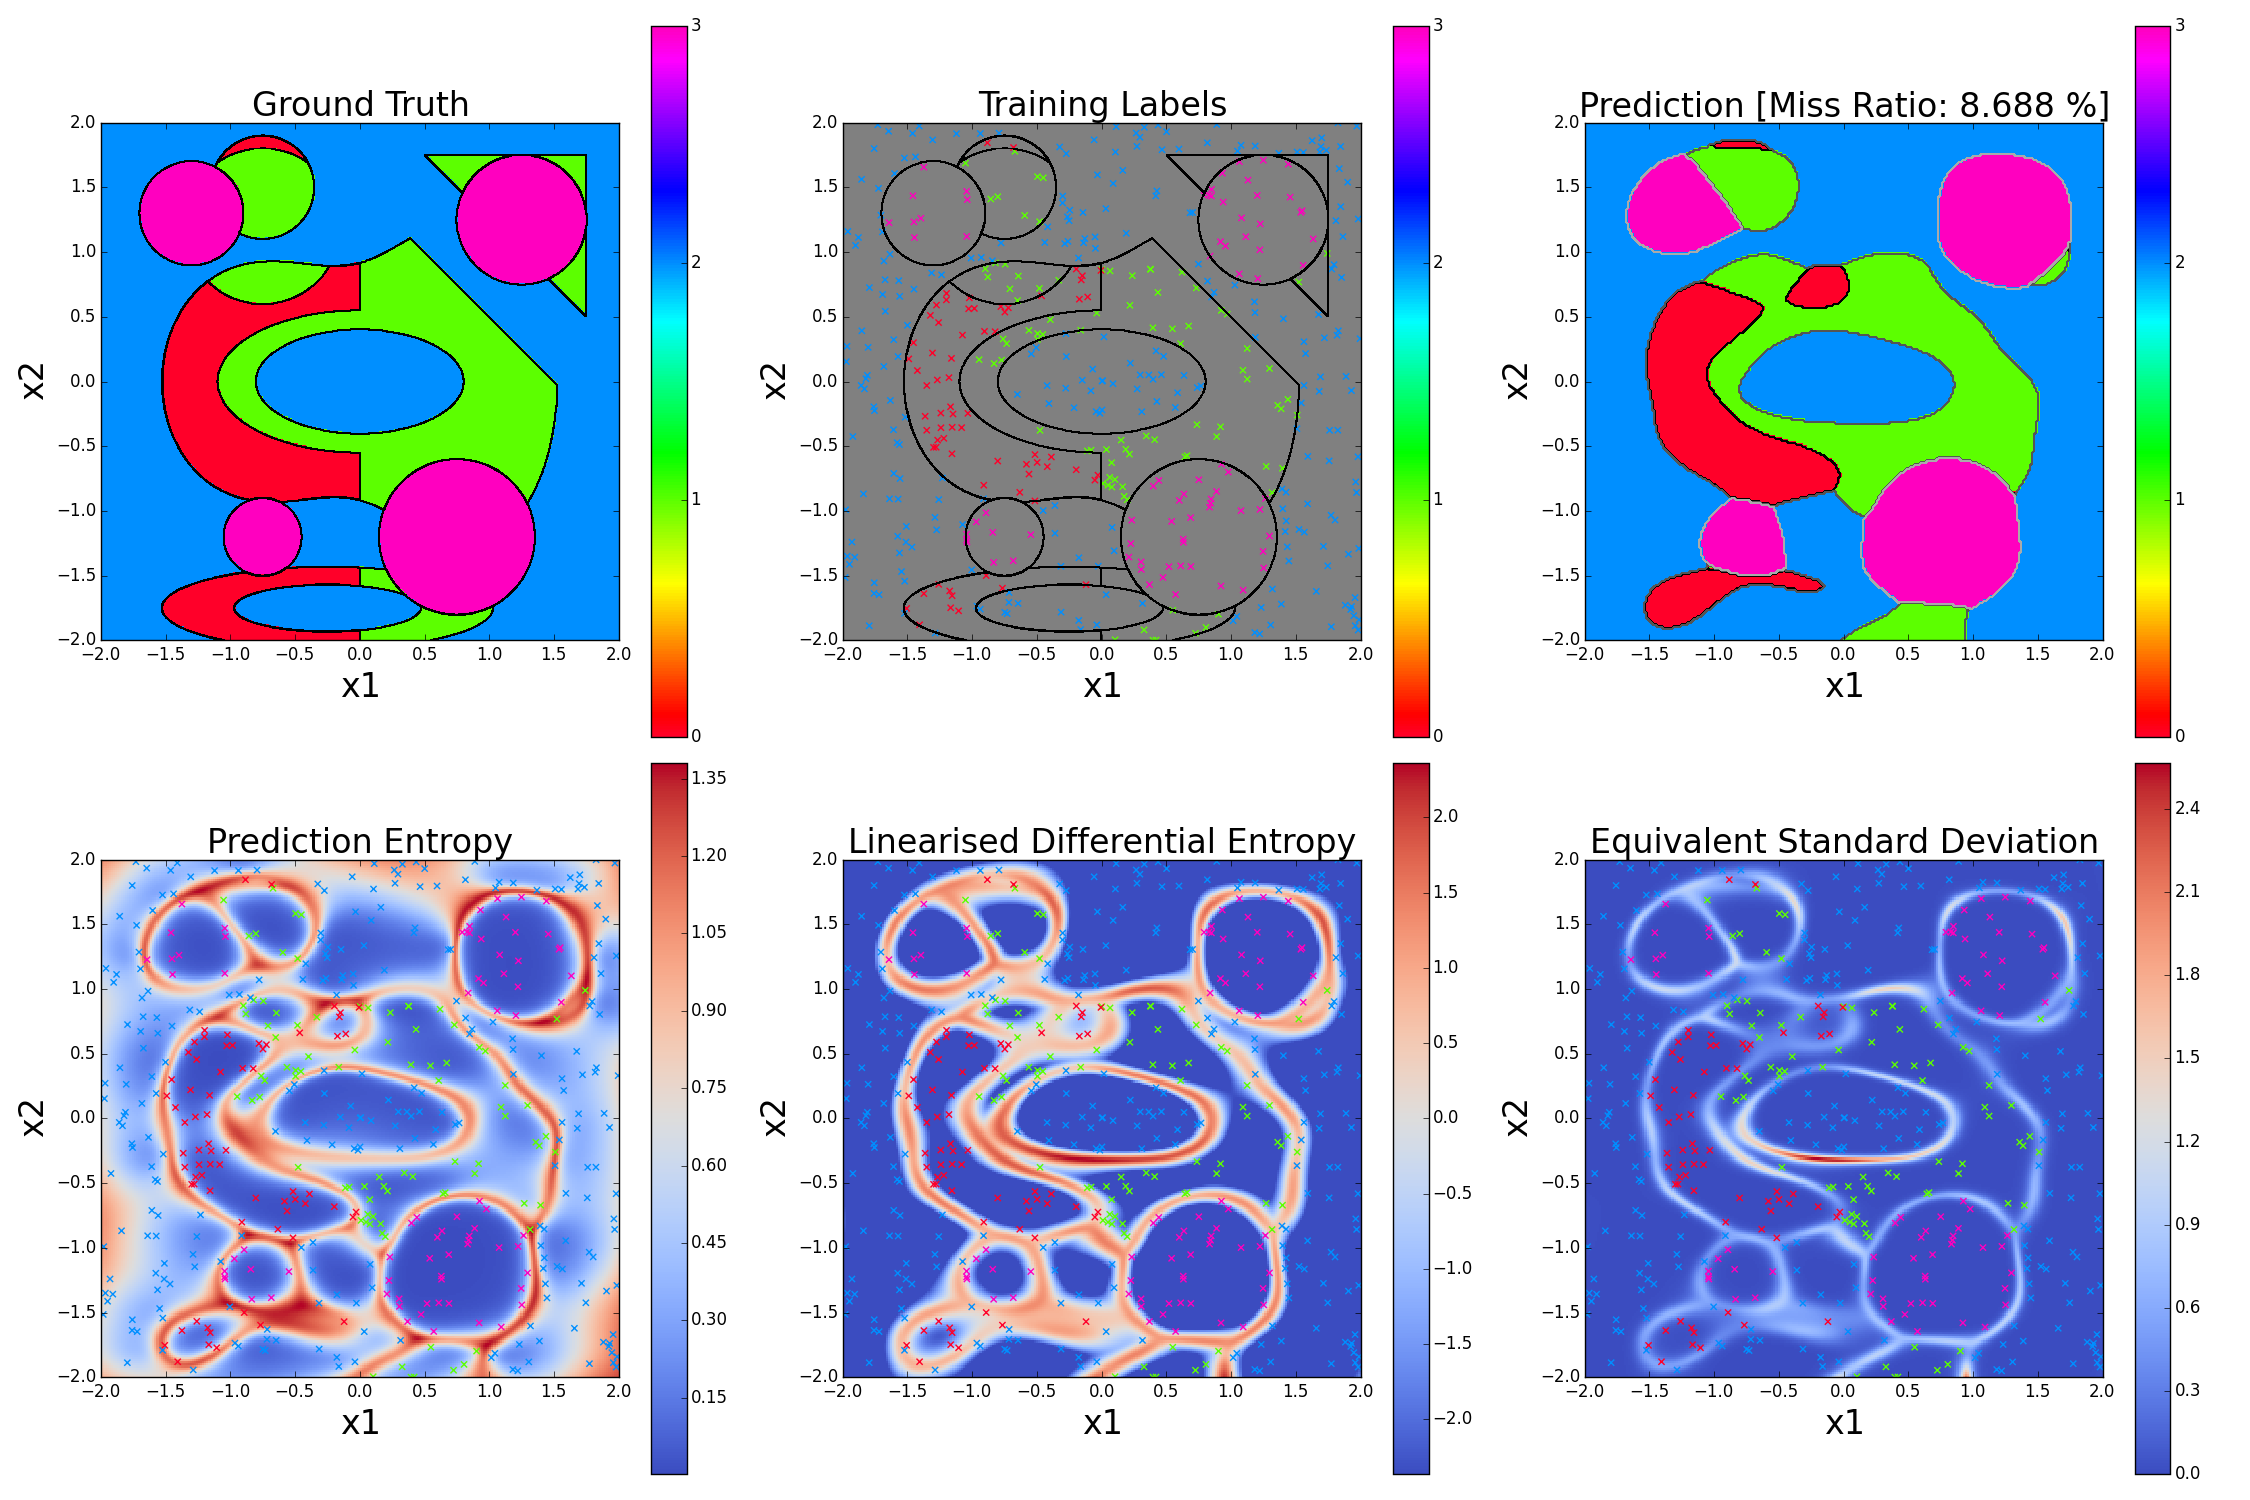
\includegraphics[width = \linewidth]{Figures/multiclass_linearised_entropy/Figure1.png}
			\caption{Example: Linearised Entropy for a Multiclass Classifier}
			\label{Figure:Results:MulticlassyLinearisedEntropy}
			\end{figure*}
					
	\subsection{Multiclass Classification}
	
		For multiclass classification, linearisation is performed on the softmax response functions which returns the predictive class probability $\vec{\pi}^{m}$ for each of the $c$ classes \eqref{Section:LinearisedEntropy:Equation:Softmax}. For notational clarity we move the query star ($^\star$) to the left and use the superscript $m$ to index the classes. The latent vector $\bvec{f}_{i}$ represents the collection of $c$ latent values across classes at the query point $i$, and is distinct from $\vec{f}_{m}$ which represents the collection of $n^{\star}$ latent values across query points for class $m$.

		\begin{equation}
			^{\star}\pi^{m}_{i} = \sigma(^{\star}\bvec{f}_{i}) := \frac{\exp(^{\star}f^{m}_{i})}{\sum_{k = 1}^{c} \exp(^{\star}f^{k}_{i})} \qquad m \in \{1, 2, \dots, c\}
		\label{Section:LinearisedEntropy:Equation:Softmax}
		\end{equation}	
					
\section{Receding Horizon Approach to Informative Path Planning}
\label{Section:RecedingHorizonApproach}

\section{Conclusions and Future Work}
\label{Section:Conclusion}

\section*{Acknowledgments}


%% This section was initially prepared using BibTeX.  The .bbl file was
%% placed here later
%\bibliography{publications}
%\bibliographystyle{named}
%% The file named.bst is a bibliography style file for BibTeX 0.99c

\bibliographystyle{named}
\bibliography{acra2015}

\end{document}

